\documentclass[12pt]{report}

% --- Packages ---
\usepackage{amsmath}
\usepackage{amsfonts}
\usepackage{amssymb}
\usepackage{amsthm}
\usepackage{graphics}
\usepackage{graphicx}
\usepackage{hyperref}
\usepackage{xcolor}
\usepackage{dblfnote}
\usepackage{enumitem}
\usepackage[backend=biber, style=ieee]{biblatex}

% --- Dictionaries Setup ---
\usepackage[xindy, nonumberlist]{glossaries}

\setglossarystyle{list}

\newglossary[alg]{en-fa}{acn}{acr}{واژه‌نامه انگلیسی به فارسی}
\newglossary[blg]{fa-en}{blo}{bls}{واژه‌نامه فارسی به انگلیسی}

\GlsSetXdyLanguage[en-fa]{english}
\GlsSetXdyLanguage[fa-en]{persian}

\makeglossaries
\loadglsentries{dictionary/dictionary}

% --- Xepersian Setup ---
\usepackage{xepersian}
\settextfont{Nazli}
\setlatintextfont{Linux Libertine O}

% --- Layout ---
\usepackage[margin=2cm]{geometry}

% --- Colors ---
\definecolor{dracbg}{HTML}{282A36}
\definecolor{link}{rgb}{0.82, 0.41, 0.12}
\definecolor{cite}{rgb}{1.0, 0.22, 0.0}
\definecolor{ToC}{rgb}{0.0, 0.34, 0.25}

% --- Bibliography/Hyperlink Setup ---
\addbibresource{bib/crypto_ref.bib}
\hypersetup{
    colorlinks=true, 
    linkcolor=link, 
    citecolor=cite, 
    urlcolor=link
}

% --- Theorems ---
\newtheorem{thm}{قضیه}[chapter]
\newtheorem{cor}[thm]{نتیجه}
\newtheorem{defn}[thm]{تعریف}
\newtheorem{prop}[thm]{گزاره}
\newtheorem{lmm}[thm]{لم}
\newtheorem{conj}[thm]{حدس}
\newtheorem{exm}[thm]{مثال}
\newtheorem{rem}[thm]{تذکر}
\newtheorem{note}[thm]{یادداشت}
\newtheorem{alg}[thm]{الگوریتم}

% --- Line Spacing ---
\linespread{1.5}

\begin{document}

% --- Title Page ---
\thispagestyle{empty}
\begin{titlepage}
    \centering
    
    {
\includegraphics[height=100pt, width=100pt]{Pics/Logo.png}\par}
    
    \vspace*{0.5cm}
    
    { پردیس علوم \par}
    { دانشکده ریاضی، آمار و علوم کامپیوتر \par}
    
    \vspace*{2cm}
    
    {\huge \bfseries رمزنگاری بر پایه سیستم های آشوبناک \par}
    
    \vspace*{2cm}
    
    { نگارنده \par}
    {\Large \textbf{علی زارع مهرجردی} \par}
    
    \vspace*{1.5cm}
    
    { استاد راهنما \par}
    {\Large غلامرضا رکنی لموکی \par}
    
    \vspace*{2cm}
    
    { پایان نامه برای دریافت درجه کارشناسی \par}
    \vspace*{0.5cm}
    { در رشته ریاضیات و کاربردها \par}
    
    \vspace*{0.5cm}
    
    { بهار ۱۴۰۵ \par}

\end{titlepage}

% --- Esalate Asar --- 
\newpage
\thispagestyle{empty}
\begin{center}
    
\includegraphics[width=100pt, height=100pt]{Pics/Logo.png}
    
    \vspace{0.6cm}
    {\large بسمه تعالی}
    
    \vspace{1.5cm}
    {\Large \textbf{تعهدنامه اصالت اثر}}
\end{center}

\vspace*{1.2cm}

\noindent
اینجانب
علی زارع مهرجردی
گواهی و تعهد می دهم که مطالب مندرج در این 
پایان نامه، 
حاصل کار پژوهشی اینجانب است و به دستاوردهای پژوهشی دیگران که در این پژوهش از آنها استفاده شده،
مطابق مقررات و اصول مرتبط با درج منابع و مآخذ، ارجاع داده ام.
این 
پایان نامه
قبلاً برای دریافت هیچ مدرک تحصیلی دیگری ارائه نشده است.
ضمن پایبندی به رعایت مقررات و اصول اخلاق در پژوهش، می پذیرم که در هر زمانی، خلاف این گواهی اثبات شود،
دانشگاه تهران حق دارد مدرک تحصیلی صادرشده را از درجه اعتبار ساقط نماید.

\vspace*{0.8cm}

\noindent
کلیه حقوق مادی و معنوی این اثر متعلق به دانشگاه تهران است.

\vspace*{2.5cm}

\begin{flushleft}
    \begin{minipage}{0.45\textwidth}
        نام و نام خانوادگی دانشجو: علی زارع مهرجردی \\[0.8cm]
        امضاء: \\[0.8cm]
        تاریخ:
    \end{minipage}
\end{flushleft}

% --- Abstract - Persian ---

\chapter*{}
\section*{چکیده}
\thispagestyle{empty}
در دنیای مدرن و در حوزه برقراری ارتباطات به صورت دیجیتال همواره مسئله
امنیت اطلاعات
نیز به صورت گره خورده با پیشرفت
تکنولوژی و همقدم با آن وجود داشته است. در حوزه امنیت اطلاعات نیز مبحث رمزنگاری همواره در بطن این حوزه قرار دارد.
امروزه سیستم های رمزنگاری مخصوصا آن دسته که به طور روزمره استفاده میشوند با اتکا بر مسئله
لگاریتم گسسته\LTRfootnote{Discrete Logarithm}
در
نظریه اعداد
و گاها همنوع های آن در حوزه
های دیگر مانند
هندسه جبری
هستند.
از این رو بررسی سیستم هایی که صرفا مبتنی بر این ساختار ها هستند همواره درحال بررسی هستند و در نتیجه سیستم هایی که بیشتر نوآورانه هستند
و از شاخه های دیگیری از ریاضیات استفاده میشوند نیز خالی از لطف نیست.
\\
در ادامه قصد داریم سیستم رمزی بر پایه
سیستم های آشوبناک\LTRfootnote{Chaotic Systems}
که در شاخه
سیستم های دینامیکی\LTRfootnote{Dynamical Systems}
ریاضی قرار میگیرند و از این منظر
نگرشی نوآورانه تر دارد را بررسی میکنیم با شروع از تئوری ریاضی و بررسی مسئله تضمین کننده امنیت این سیستم و درنهایت نیز مقایسه ای با 
سیستم های متعارف که امروزه مانند
\lr{RSA}\LTRfootnote{Rivest–Shamir–Adleman}
در دنیای دیجیتال استفاده میشود خواهیم داشت و در همین بخش نقاط ضعف و قوت این سیستم را به تفضیل بررسی خواهیم کرد.

\vspace*{\fill}

\textbf{ کلمات کلیدی:  }
سیستم رمز،  سیستم آشوبناک، سیستم های دینامیکی

% --- Table of Contents --- 

\newpage
\pagestyle{plain}
\setcounter{page}{1}
\pagenumbering{harfi}

% --- Table of Contents ---
{
\hypersetup{linkcolor=ToC}
\tableofcontents
}

\newpage

% --- List of Figures ---
\listoffigures

% --- Acknowledgement page ---
\chapter*{سپاسگزاری}
\section*{سپاسگزارم}

% --- Pishgoftar ---
\chapter*{پیشگفتار }
پیش گفتار

\chapter{ مفاهیم مقدماتی  }
% --- Page Numbering Setup ---
\setcounter{page}{1}
\pagenumbering{arabic}

در این فصل مفاهیم پایه ای مورد نیاز برای ادامه مسیر معرفی شده و به بررسی و نوع استفاده از آنها میپردازیم.
به اصل
کِرک‌هُوفس
نگاهی خواهیم انداخت و اصول ششگانه آن را مطرح میکنیم موارد منسوخ شده و اصل دوم آن که همواره جزء مهمترین اصول
سیستم های رمزنگاری مدرن جهان است را بررسی میکنیم و به معنای آن خواهیم پرداخت.

% --- Section: Cryptosystem ---
\section[ سیستم رمز  ]{ سیستم رمز\LTRfootnote{Cryptosystem}}
یک سیستم رمز به شکل یک پنج تایی مرتب
\eqref{eq:crypto}
معرفی میشود که به تعریف اعضای آن به ترتیب عبارت هستند از: \\
فضای متن آشکار\LTRfootnote{Plaintex Space}
$(\mathcal{P})$
\lr{--}
فضای متن رمزشده\LTRfootnote{Ciphertex Space}
$(\mathcal{C})$
\lr{--}
فضای کلید\LTRfootnote{Key Space}
$(\mathcal{K})$
\lr{--}
تابع رمزکننده\LTRfootnote{Encryption Function}
$(E)$
\lr{--}
تابع رمزگشا\LTRfootnote{Decryption Function}
$(D)$


\begin{equation}
    \left( \mathcal{P}, \mathcal{C}, \mathcal{K}, E, D \right)  \label{eq:crypto}
\end{equation}
ابتدا تعریف مختصری برای هرکدام از اصطلاحات استفاده شده ارائه میدهیم.

\subsection[فضای متن آشکار]{فضای متن آشکار}
\label{sec:plaintext-space}
هنگامی که قصد داریم پیامی را به صورت رمز شده مخابره کنیم، پیام خام قبل از رمز شدن یا به عبارتی دقیقا
عبارتی که نویسنده آن را تولید میکند فارغ از آنکه چه چیزی باشد در فضای متن آشکار
(\lr{Plaintext})
قرار میگیرد.
این فضا متشکل از تمام حالت های قرار گیری حروف الفبای مورد استفاده در کنار هم به هر طول دلخواهی است.
فرضا از حروف الفبای فارسی استفاده کنیم، تمام دنباله های ساخته شده بوسیله  ۳۲ حرف فارسی به اضافه علائم نگارشی در این فضا قرار میگیرند.
از آنجایی که الفبای مورد استفاده غیرتهی است، این فضا واضحا همواره نامتناهی است.

\subsection[ فضای متن رمزشده  ]{ فضای متن رمزشده }
این فضا شامل تمام متن های موجود در بخش قبلی
(\ref{sec:plaintext-space})
به صورت رمزشده است.
به عبارت دیگر فضاي متن آشکار توضیح داده شده در بخش قبل را درظر بگیرید که شامل تمامی متن های قابل تولید با حروف الفبای مورد استفاده بود.
اگر تمامی آن متن ها را با کمک سیستم رمز کنیم و در یک مجموعه جدید قرار دهیم تشکیل مجموعه فضای متن رمزشده را میدهد.

\subsection[ فضای کلید  ]{ فضای کلید }
فضای کلید، به مجموعه ای از تمامی کلید هایی که میتوانند در
\hyperref[subsec:encryption-function]{ تابع رمزکننده }
و همچنین
\hyperref[subsec:decryption-function]{ تابع رمزگشا }
استفاده شوند، گویند.

\subsection[ تابع رمزکننده  ]{ تابع رمزکننده }
\label{subsec:encryption-function}
به تابعی که متن اولیه را بعنوان ورودی دریافت کرده و به کمک یک کلید یکسان
(در سیستم های متقارن\LTRfootnote{Symmetric})
و یک کلید مخصوص
(در سیستم های نامتقارن\LTRfootnote{Asymmetric})
متن رمز شده را تولید میکند تابع مرزکننده گویند.

\subsection[ تابع رمزگشا  ]{ تابع رمزگشا }
\label{subsec:decryption-function}
به تابعی که متن رمز شده را بعنوان ورودی دریافت کرده و به کمک یک کلید یکسان
(در سیستم های متقارن)
و یک کلید مخصوص
(در سیستم های نامتقارن)
متن اولیه را تولید میکند، تابع رمزگشا گویند.

\newpage

% --- Section: Kerckhoffs ---
\section[ اصل کِرک‌هُوفس - \lr{Kerckhoffs} ]{ اصل کِرک‌هُوفس}
\label{sec:kerckehoffs-principle}
آگوست کِرک‌هُوفس\LTRfootnote{Auguste Kerckhoffs}
ربان شناس و رمزنگار اهل هلند در مقاله خود به عنوان رمزنگاری مدرن
\cite{kerckhoffs-1883}
شش اصل کلی برای سیستم های رمز معرفی میکند که باید از آنها تبعیت کنند. این اصول عبارتند از:

% --- Kerckhoffs Rules ---
\begin{enumerate}[leftmargin=*]
    \item[1]
        سیستم رمزنگاری، اگر نه از نظر تئوری بلکه در عمل غیرقابل شکست باشد.
    \item[\textcolor{red}{$\ast$}] \label{item:kerckhoffs}
        سیستم رمزنگاری باید هیچ نکته پنهان ومحرمانه ای نداشته باشد بلکه تنها چیزی که باید محرمانه نگه داشته شود کلید رمز است،
        طراح سیستم رمزنگار نباید جزئیات سیستم خود را حتی از دشمنان پنهان کند.
        (\hyperref[sec:kerckehoffs-principle]{  اصل کِرک‌هُوفس } )
    \item[3]
        کلید رمز باید به گونه ای قابل انتخاب باشد که اولاً بتوان آن را به راحتی عوض کرد و ثانیاً بتوان آن را به خاطر سپرد
        و نیازی به یادداشت کردن کلید رمز نباشد.
    \item[4]
        متون رمزنگاری شده باید با تلگراف قابل مخابره باشد.
    \item[5]
        دستگاه رمزنگاری یا اسناد رمزشده باید برای یک نفر قابل حمل باشند.
    \item[6]
        سیستم رمزنگاری باید به آسانی قابل راه اندازی و کاربری باشند چنین سیستمی نباید به آموزش های مفصل و رعایت 
        فهرست بزرگی از قواعد و دستورالعمل ها نیاز داشته باشد.
\end{enumerate}

هرچند که برخی از این اصول با توجه به پیشرفت تکنولوژی، امروزه منسوخ است اما
\hyperref[item:kerckhoffs]{ اصل دوم  }
همواره از نظر فعالان این حوزه مورد قبول و به عنوان یکی از اصول بنیادین در زمینه رمزنگاری نامبرده میشود.
به طوری که تقریبا غیرممکن است که کتابی استاندارد درحوزه رمزنگاری پیداکنید بدون آنکه در آن به این اصل اشاره کرده باشد.
با اتکا برهمین اصل است که امروزه عموما از سیستم های رمزی استفاده میشود که ساختار کلی آنها به طور 
«متن باز»\LTRfootnote{Open-Source}
در اختیار عموم قرار دارد.
\\\noindent
به هنگام استفاده از سیستم های رمز با توجه به امن بودن کانال انتقال و یا ناامن بودن کانال انتقال 
در حالت کلی دو دسته سیستم رمز داریم که در بخش بعدی به بررسی آنها و موارد استفاده
و معنای امن بودن کانال انتقال خواهیم پرداخت.

\newpage

% --- Section: Symmetric & Asymmetric ---
\section{ رمزنگاری متقارن و نامتقارن  }
به هنگام انتقال پیام ها و گاها کلید ها از بستری این امر فراهم میشود که به این بستر کانال ارتباطی گفته میشود.\\
اگر این کانال به صورت تضمین شده غیرقابل شنود باشد و فقط شخص فرستنده و گیرنده از محتوای ارسالی مطلع باشند، به این کانال یک کانال امن میگوییم.
در غیر این صورت حتی اگر تهدید و ریسک شنود نیز موجود باشد کانال ناامن درنظر گرفته میشود.
\\\noindent
در دنیای واقعی چون تامین امنیت کامل برای یک کانال بسیار سخت و گاها هزینه بر هست عموما فرض بر ناامن بودن کانال ارتباطی گرفته میشود.
حتی اگر در سازمان بخصوصی کانال ارتباطی داخلی درنظر گرفته بشود با تمامی م تدابیر امنیتی سازمان
همواره امنیت این زنجیره (کانال ارتباطی) به اندازه ضعیف ترین عنضرش خواهد بود، و امکان نشست اطلاعات از هرکدام از کارکنان سازمان
وجود دارد. برای همین است که عموما فرض بر ناامن بودن کانال ارتباطی مورد نظر قرار میگیرد.

\subsection[ رمزنگاری متقارن ]{ رمزنگاری متقارن  }
\label{subsec:symmetric-cryptography}
این سیستم همانطور که از نام آن قابل انتظار است برای رمزگشایی و رمزنگاری از یک کلید استفاده میکند.
همانطور که در تصویر
\ref{fig:symmetric-cryptography}
مشاهده میکنید بخاطر استفاده از تک کلید در این سیستم حالت متقارن را به ارمغان می‌آورد.

% --- Fig: Symmetric_Cryptography ---
\begin{figure}[h]
    \centering
    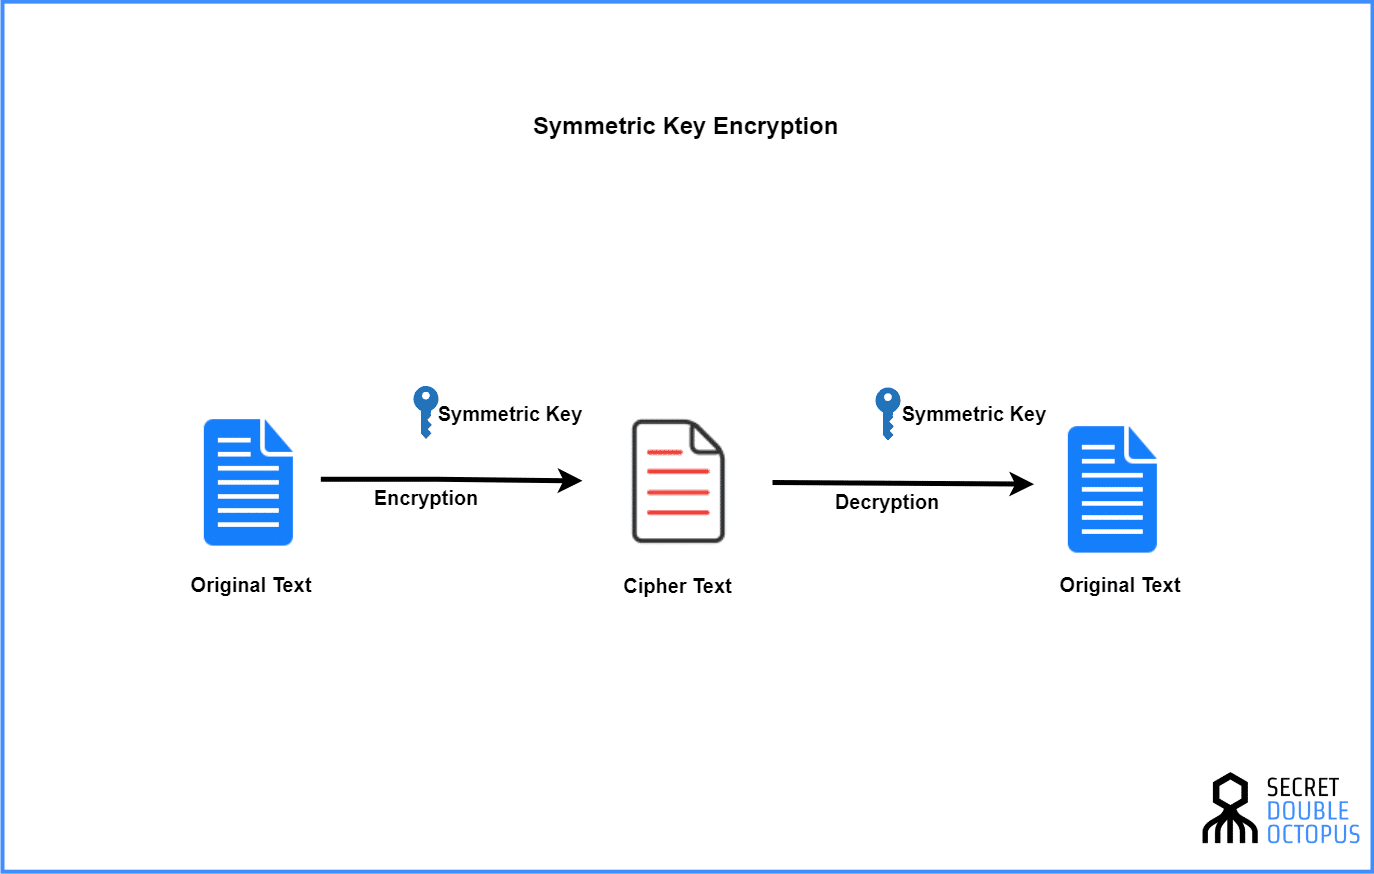
\includegraphics[width=0.5\textwidth, height=5cm]{Pics/Symmetric_Cryptography.png}
    \caption{%
        تصویر شماتیک سیستم رمزنگاری متقارن، تصویر گرفته شده از
        \href{https://doubleoctopus.com/security-wiki/encryption-and-cryptography/symmetric-key-cryptography/}{Secret-Double-Octopus}
    }
\end{figure}\label{fig:symmetric-cryptography}
\noindent
استفاده از این سیستم در کانال های ناامن هرگز توصیه نمیشود چراکه درکانال های ارتباطی ناامن امکان لو رفتن کلید وجود دارد
و همانطور که در توضیحات مطالعه کردیم، در این سیستم ها کلید برای رمز کردن و کلید برای رمزگشایی یکسان است.
و در صورتی که کلید رمزنگاری لورفته باشد تمام امنیت سیستم ازبین رفته است.
موارد مثال این نوع سیستم عبارت‌اند از:
(\lr{ DH\LTRfootnote{Diffie-Hellman}, AES\LTRfootnote{Advanced-Encryption-System} }).

\subsection[ رمزنگاری نامتقارن ]{ رمزنگاری نامتقارن  }
این سیستم نیز با توجه به اسم آن نمایانگر سیستمی نامتقارن است.
عاملی که این تقارن در سیستم را برهم میزند وجود دوکلید در سیستم است. بر خلاف رمزنگاری
\hyperref[subsec:symmetric-cryptography]{متقارن}
که برای هردو رمزنگاری و رمزگشایی از یک کلید یکسان استفاده میشود.
در این سیستم که خصوصا در کانال های ارتباطی ناامن مزیت خود را نشان میدهد دو کلید توسط شخص ایجاد میشود
که آنها کلید خصوصی و کلید عمومی نامیده میشوند در ادامه هرکدام را جداگانه توضیح خواهیم داد:
\subsection*{ کلید عمومی }
این کلید به صورت عمومی منتشر میشود و در کانال ارتباطی قرار میگیرد یعنی هر کسی حتی شخص شنودگر نیز امکان دسترسی به آن را دارد
تنها کاری که این کلید انجام میدهد رمز کردن محتوای مورد نظر فرستنده خواهد بود و در رمزگشایی هیچ عملکردی نخواهد داشت 
پس هنگامی که فرستنده متن را به کمک این کلید رمز میکند و محتوای رمز شده را در کانال فرضا حتی ناامن قرار میدهد حتی فرد شنودگر که 
دسترسی به محتوای رمزشده و کلید عمومی دارد هیچ کمکی در راستای رمزگشایی متن به او نخواهد کرد.

\subsection*{ کلید خصوصی }
این کلید که نزد فرد دریافت کننده است برای رمزگشایی متن رمز شده توسط کاربر است البته در سیستم هایی مانند 
\lr{RSA}
با دراختیار داشتن کلید خصوصی تمام سیستم برای فرد لو میرود یعنی اطلاعات کامل سیستم را خواهد داشت چه برای رمز کردن چه برای رمزگشایی.
\noindent
در تصویر زیر شمای کلی سیستم رمزنگاری نامتقارن آورده شده است.
\begin{figure}[h]
\centering
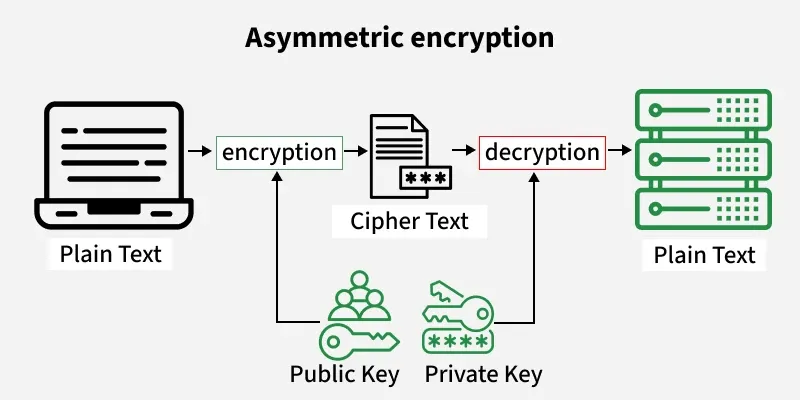
\includegraphics[width=0.5\textwidth]{Pics/Asymmetric_Cryptography.png}
\caption{%
تصویر شماتیک سیستم رمزنگاری نامتقارن، تصویر گرفته شده از
\href{https://www.geeksforgeeks.org/computer-networks/what-is-asymmetric-encryption/}{Geek-for-Geeks}
}
\end{figure}

\chapter{ سیستم رمزنگاری باپتیستا  }

\chapter{ تحلیل امنیت و آسیب پذیری  }

\chapter{ راهکار های مقابله و مقایسه  }

\chapter{ پیاده سازی و آزمایش های عددی  }

\chapter{نتیجه گیری}

% --- Dictionaries ---
\glsaddall

\printglossary[type=en-fa]
\printglossary[type=fa-en]

\newpage

% --- References ---
\phantomsection
\addcontentsline{toc}{chapter}{منابع}
\nocite{*}
\begin{latin}
    \printbibliography
\end{latin}

% --- Abstract - English ----
\begin{latin}
    \chapter*{Abstract}
    Abstract goes here...
\end{latin}

\newpage
\thispagestyle{empty}

% --- Title Page - English --- 
\begin{latin}
\begin{figure}
\centering

\includegraphics[height=100pt, width=100pt]{Pics/Logo.png}
\end{figure}
\begin{center}

College of Science\\
School of Mathematics, Statistics, and Computer Science
\end{center}

\begin{center}
%%%%%%%%%%%%%
\end{center}

\begin{center}
\huge{Cryptography based on chaotic systems}
\end{center}

\begin{center}
%%%
\end{center}

\begin{center}
\textbf{
Ali Zaremehrjardi
}
\end{center}

\begin{center}
    Supervisor \\[1ex]
Gholamreza Rokni Lamouki
\end{center}

\vspace{3cm}
\begin{center}
    A thesis submitted in partial fulfillment of the requirements for \\[1ex]
the degree of B.Sc. in Mathematics and applications
\end{center}

\begin{center}
Spring 2026
\end{center}

\end{latin}

\end{document}
